\documentclass[11pt,a4paper]{article}
\usepackage[margin=20mm]{geometry}
\usepackage{amsmath,amssymb,booktabs,graphicx,float,hyperref,fancyhdr}
\hypersetup{colorlinks=true,urlcolor=blue,linkcolor=blue}
\pagestyle{fancy}\fancyhf{}\lhead{Height distribution analysis}\rhead{Two skew-normal components}\cfoot{\thepage}
\setlength{\headheight}{14pt}\setlength{\parindent}{0pt}\setlength{\parskip}{6pt}
\graphicspath{{./}{assets/data/}}
\begin{document}
\begin{center}{\LARGE Statistical analysis of heights}\\[5pt]
{\large Two-component skew-normal mixture}\\[4pt]
Executed in Python; 2 November 2026\end{center}
\section*{Interpretation}
The constrained best fit has two local maxima. This is a possible descriptive
representation, but the data do not establish a stable two-peaked population.
The second component's shape reaches its upper bound, indicating sensitivity
to nearly one-sided component shapes. AIC favors a two-normal mixture; BIC
favors a single normal. The seven-parameter model is not the preferred model
under either criterion. Components must not be interpreted as demographic,
biological or causal groups without external evidence.

Of 200 successful observation-bootstrap refits, 191 (95.5\%) had exactly two modes. These resampling results assume independent observations; they are not a posterior probability of population bimodality.

\section*{Data inspection and preparation}
The UTF-8 CSV has a single header, \texttt{height\_cm}. With one field per line there is no observable field separator to distinguish comma from other delimiters; comma parsing was used. Decimal formatting uses a point (153.5). There are 109 original data records, 109 retained finite numeric records, and 0 missing/invalid records. No exclusions, winsorization, outlier removal or substantive transformations were performed. Repeated values were preserved. The computational standardization $z=(x-169.56422018)/9.13405840$ is inverted in all reported parameters.

\begin{center}
\small
\begin{tabular}{lr}
\toprule
Statistic & Value\\
\midrule
Mean (cm) & 169.56422\\
Sample variance (cm squared; n-1) & 83.43102\\
Sample SD (cm; n-1) & 9.13406\\
Median (cm) & 170.00000\\
Minimum (cm) & 151.00000\\
Maximum (cm) & 191.00000\\
\bottomrule
\end{tabular}
\end{center}
\begin{center}
\small
\begin{tabular}{lr}
\toprule
Percentile & Height (cm)\\
\midrule
1 & 152.00000\\
5 & 154.40000\\
10 & 158.00000\\
25 & 162.00000\\
50 & 170.00000\\
75 & 177.00000\\
90 & 181.00000\\
95 & 182.60000\\
99 & 185.92000\\
\bottomrule
\end{tabular}
\end{center}
There are 35 distinct values; 108/109 observations are integer centimetres. Rounding/heaping is substantial. Sample percentiles use NumPy linear interpolation. No dates, group labels, censoring, truncation limits or sampling design are supplied. Row-order lag-1 correlation is 0.1278; Spearman correlation with row number is 0.1547. Neither establishes independence. Repeated measurements or clustering would require an appropriate cluster/block bootstrap with metadata.

\clearpage
\section*{Model and estimation}
For real $x$, the fitted model is
\[
 f(x)=w f_{\rm SN}(x;\xi_1,\omega_1,\alpha_1)
 +(1-w)f_{\rm SN}(x;\xi_2,\omega_2,\alpha_2),\qquad
 f_{\rm SN}(x;\xi,\omega,\alpha)=\frac{2}{\omega}\phi(z)\Phi(\alpha z),
 \quad z=\frac{x-\xi}{\omega}.
\]
Here $\phi(z)=(2\pi)^{-1/2}\exp(-z^2/2)$ and
$\Phi(z)=\int_{-\infty}^z\phi(t)\,dt$ are the standard-normal density and CDF.
$\xi$ is a location (cm), $\omega>0$ is a scale (cm); they are generally
not the component mean and standard deviation. Shape $\alpha$ and weight $w$
are dimensionless. Two components do not automatically imply two modes.
The fit was not required to be bimodal.

All seven parameters were jointly optimized against the individual observations.
The log-likelihood is $\ell=\sum_i\log\{wf_1(x_i)+(1-w)f_2(x_i)\}$.
Calculations use normal log-CDFs, stable log-sum-exp, analytic gradients,
log-scales and bounded L-BFGS-B. Analytic gradients were checked against
finite differences (maximum discrepancy $6.8\times10^{-9}$ at an interior point).
This is a best-found constrained likelihood maximum, not a proof of a global
unconstrained maximum.

\textbf{All bounds.} For each component, $71\leq\xi\leq271$ cm,
$1\leq\omega\leq160$ cm, $-20\leq\alpha\leq20$, and
$0.03\leq w\leq0.97$. There is no additional penalty. The location bounds are
the sample range expanded by twice its width; the upper scale is four times
the range. These are broad numerical guards. The 1 cm scale floor corresponds
to the predominant recording increment and prevents arbitrarily narrow
components at repeated observations; it is a modeling choice, not an estimated
measurement-error SD. The weight floor limits tiny fitted groups to roughly
three observations at this sample size. Bounds are frozen to the original
data in every bootstrap refit. Shape caps limit extreme one-sided fits and
are checked below. Scale floors 0.5 and 2 cm are also investigated.

The primary fit used seed 20261102, 160 starts with quantile-separated/overlapping locations, random scales and weights, and mixed positive, zero and negative shapes. 160 starts converged; 11 converged within 0.01 log-likelihood units of the best. The worst converged log-likelihood was -398.591148, versus -389.078835 for the best. Thus competing starts can reach materially inferior local solutions. The best used 82 iterations.

The best optimizer run stopped on the relative function-reduction criterion (the exact message is in JSON). Active bound: second (higher-mean) component shape $\alpha_2=20$. The raw gradient infinity norm is 0.124238; at an active constraint it need not vanish. All other primary bounds are inactive. Full per-start likelihoods are saved in the JSON results. Convergence is the optimizer criterion, not a guarantee of global optimality.

\section*{Rounding and sampling limitations}
The analysis maximizes continuous densities at the reported values, as requested.
A rounded-data likelihood integrating over measurement intervals could alter
the sharp valley near common recorded heights; it was not fitted because the
measurement protocol is unknown. No jitter was added. Independence is plausible
only as a working cross-sectional assumption: it cannot be verified from
this one-column file. No evidence in the file establishes selection limits,
truncation or censoring. The empirical extrema are not physical support bounds.

\clearpage\section*{Parameters and moments}
\begin{center}
\small
\begin{tabular}{lrrrr}
\toprule
Component & Weight & Location (cm) & Scale (cm) & Shape\\
\midrule
1.00000 & 0.44432 & 166.73491 & 7.49606 & -3.79735\\
2.00000 & 0.55568 & 169.59828 & 8.22341 & 20.00000\\
\bottomrule
\end{tabular}
\end{center}
\begin{center}
\small
\begin{tabular}{lrr}
\toprule
Component & Actual mean (cm) & Actual SD (cm)\\
\midrule
1.00000 & 160.95111 & 4.76850\\
2.00000 & 176.15143 & 4.96797\\
\bottomrule
\end{tabular}
\end{center}
Labels are ordered by actual component mean, including in every bootstrap fit.
For $\delta_j=\alpha_j/\sqrt{1+\alpha_j^2}$,
\[
 m_j=\xi_j+\omega_j\delta_j\sqrt{2/\pi},\quad
 v_j=\omega_j^2(1-2\delta_j^2/\pi),\quad
 \mu=\sum_jw_jm_j,\quad V=\sum_jw_j\{v_j+(m_j-\mu)^2\}.
\]

The mixture mean is 169.397656 cm, variance 80.863867 cm$^2$, and SD 8.992434 cm. Sample mean and sample SD ($n-1$) are 169.564220 and 9.134058 cm. The model variance is a population moment and is not corrected by $n/(n-1)$.

\textbf{Complete fitted density.} For $x$ measured in cm, define $z_1=(x-166.73490936)/7.49606304$ and $z_2=(x-169.59828286)/8.22340771$. Then

\[ f(x)=0.44431760\frac{2}{7.49606304}\phi(z_1)\Phi(-3.79734760z_1) + 0.55568240\frac{2}{8.22340771}\phi(z_2)\Phi(20.00000000z_2)\]

Density units are cm$^{-1}$. Unrounded parameters in the JSON are used for all calculations. The mathematical support is the entire real line. Heights are physically positive; fitted $P(X<0)=5.86e-110$ (negligible to numerical precision). No contextual upper physiological bound is supplied, so no invented upper-limit probability is reported.

\section*{Comparison on the same observations}
\begin{center}
\small
\begin{tabular}{lrrrr}
\toprule
Model & k & Log likelihood & AIC & BIC\\
\midrule
Normal & 2 & -395.27109 & 794.54219 & 799.92488\\
Skew-normal & 3 & -395.20543 & 796.41086 & 804.48491\\
Two normals & 5 & -390.14756 & 790.29512 & 803.75186\\
Two skew-normals & 7 & -389.07884 & 792.15767 & 810.99711\\
\bottomrule
\end{tabular}
\end{center}
AIC $=2k-2\ell$; BIC $=k\log n-2\ell$. A normal has 2 parameters,
a skew-normal 3, two normals 5 and two skew-normals 7. Normal fitting is
analytic; the skew-normal used 60 starts and two normals 100. Alternatives use
the same broad location/scale guards; shape/weight bounds apply when relevant.
The simple normal maximum is interior. AIC favors two normals, while BIC
favors the normal. The two-skew-normal gain over two normals is small for
two additional parameters. These criteria are descriptive approximations:
mixtures are nonregular and the selected shape bound is active. Nominal
parameter counts are not adjusted to make the constrained model look better.
No ordinary chi-square likelihood-ratio test for component count was used:
under the null, component parameters can be unidentified and weights lie on
a boundary. Rounding and possible dependence further limit inference.

\clearpage\section*{Numerical modes and sensitivity}
\begin{center}
\small
\begin{tabular}{lrr}
\toprule
Extremum & Height (cm) & Density (1/cm)\\
\midrule
mode & 163.52935 & 0.04091\\
valley & 168.73561 & 0.00805\\
mode & 170.64228 & 0.05417\\
\bottomrule
\end{tabular}
\end{center}
The valley density is 0.197 times the lower peak density. The primary fit therefore has two distinct mathematical peaks, but the conclusion about a population remains sensitive to fitted shape and sampling variability.

The adaptive search spans 87.3642 to 251.8324 cm, extending ten scale parameters either side of every component location and including the observed range. Since each skew-normal density is at most twice its corresponding normal density, each omitted tail is bounded above by $2\Phi(-10)<1.6\times10^{-23}$. Derivative sign changes on 8,193 points were refined with Brent root finding. Repeating with 32,769 points gives the same extrema to 5.7e-14 cm. The extreme tails lie beyond all component modes; each component is monotone there. No tail peaks are hidden by the search boundary.

\begin{center}
\small
\begin{tabular}{lrr}
\toprule
Component & Mean (cm) & Component mode (cm)\\
\midrule
1 & 160.95111 & 163.52936\\
2 & 176.15143 & 170.76577\\
\bottomrule
\end{tabular}
\end{center}
Total-density modes differ from both component means and component modes.

\begin{center}
\small
\begin{tabular}{lrrrr}
\toprule
Scale floor (cm) & Shape cap & Log likelihood & Modes & Mode locations (cm)\\
\midrule
0.50000 & 20 & -389.05924 & 2 & 168.684, 180.028\\
2.00000 & 20 & -389.07884 & 2 & 163.529, 170.642\\
1.00000 & 10 & -389.52279 & 2 & 159.951, 173.874\\
1.00000 & 50 & -387.15629 & 2 & 163.806, 170.212\\
\bottomrule
\end{tabular}
\end{center}
Reducing the scale floor to 0.5 cm yields an almost equally likely solution with peaks near 168.68 and 180.03 cm. A shape cap of 10 instead gives peaks near 159.95 and 173.87 cm and an active scale floor. Thus peak positions are not robust to reasonable constraints, even though all these fits are mathematically bimodal.

Each sensitivity fit used 80 new starts plus the primary warm start. These are alternative constrained best-found solutions, with no penalty. Full sensitivity parameters and extrema are in the JSON. Active constraints by sensitivity setting:
\begin{itemize}

\item Floor 0.5 cm, shape cap 20: 6 upper.

\item Floor 2.0 cm, shape cap 20: 6 upper.

\item Floor 1.0 cm, shape cap 10: 2 lower, 3 lower.

\item Floor 1.0 cm, shape cap 50: 6 upper.

\end{itemize}
Constraint index mapping (zero based optimizer vector): 0 weight; 1,2,3 first
location, log-scale, shape; 4,5,6 second location, log-scale, shape.
Indices refer to optimizer ordering, which can differ from mean-ordered labels.
An increasing shape cap can raise likelihood through a sharper transition near
rounded observations. This is a warning about interpreting the valley literally.
Sensitivity here varies scale and shape bounds; broader weight-floor or
measurement-protocol studies are recommended, not claimed as executed.

\clearpage\section*{Density and histogram sensitivity}
\begin{center}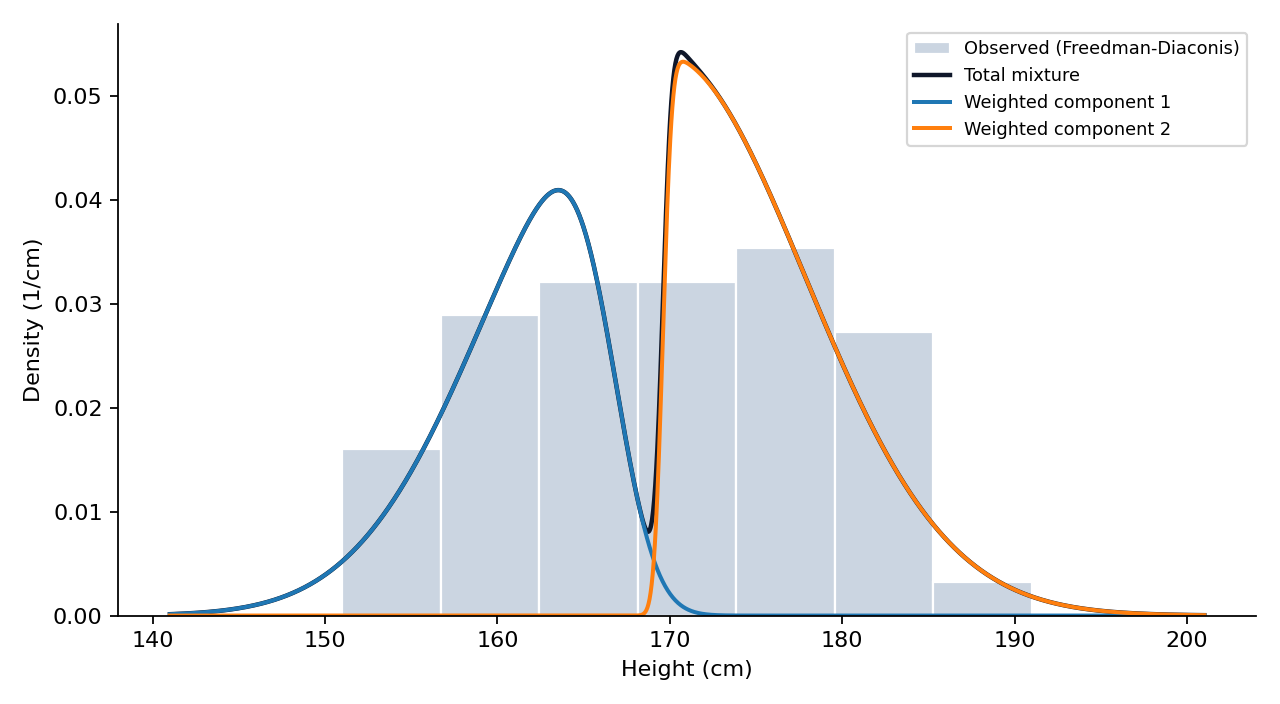
\includegraphics[width=0.96\textwidth]{heights_density.png}\end{center}
The histogram integrates to one; component curves are multiplied by their
weights and sum to the total density. Freedman--Diaconis bins are used above.
\begin{center}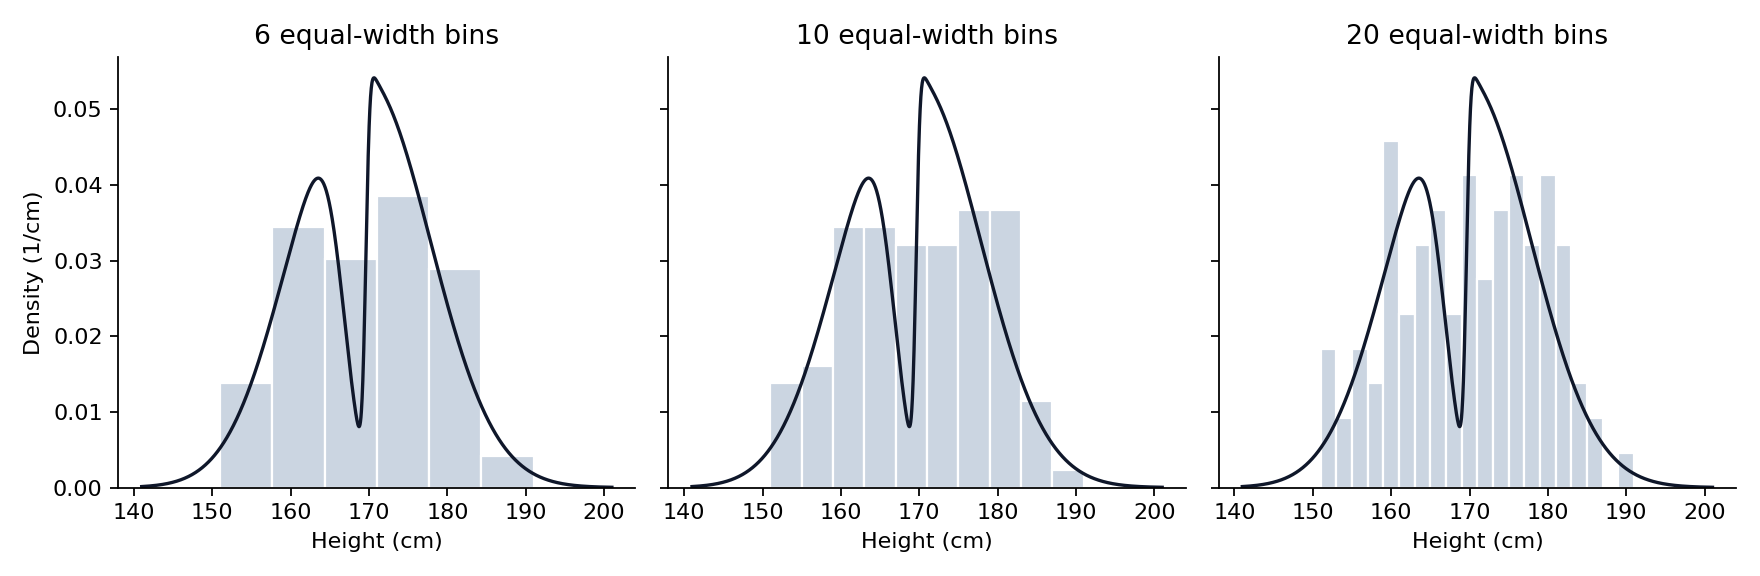
\includegraphics[width=\textwidth]{heights_bins.png}\end{center}
The same fitted curve is shown over 6, 10 and 20 equal-width bins on the same
observations. Apparent histogram peaks depend on binning and rounding. None
of these views was used to remove observations or force a bimodal fit.
No kernel density estimate was used, so there is no unreported KDE bandwidth.
\clearpage\section*{CDF and mixture Q--Q diagnostics}
\begin{center}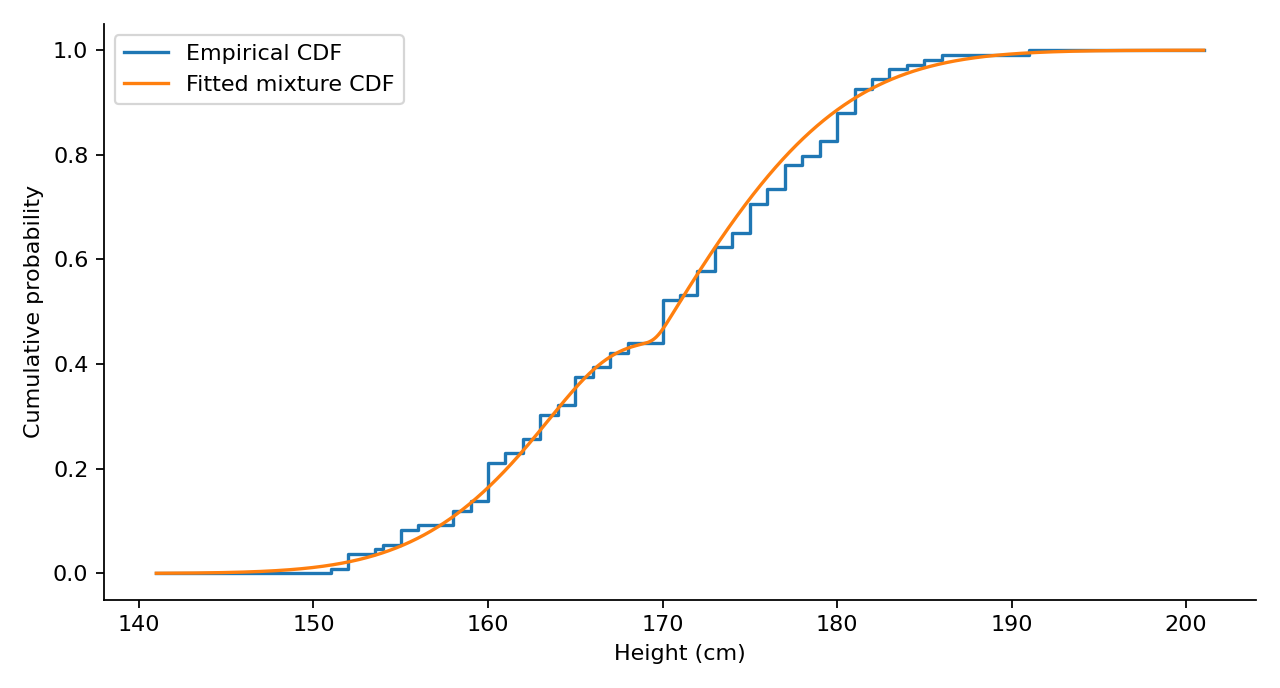
\includegraphics[width=0.85\textwidth]{heights_cdf.png}\end{center}
\begin{center}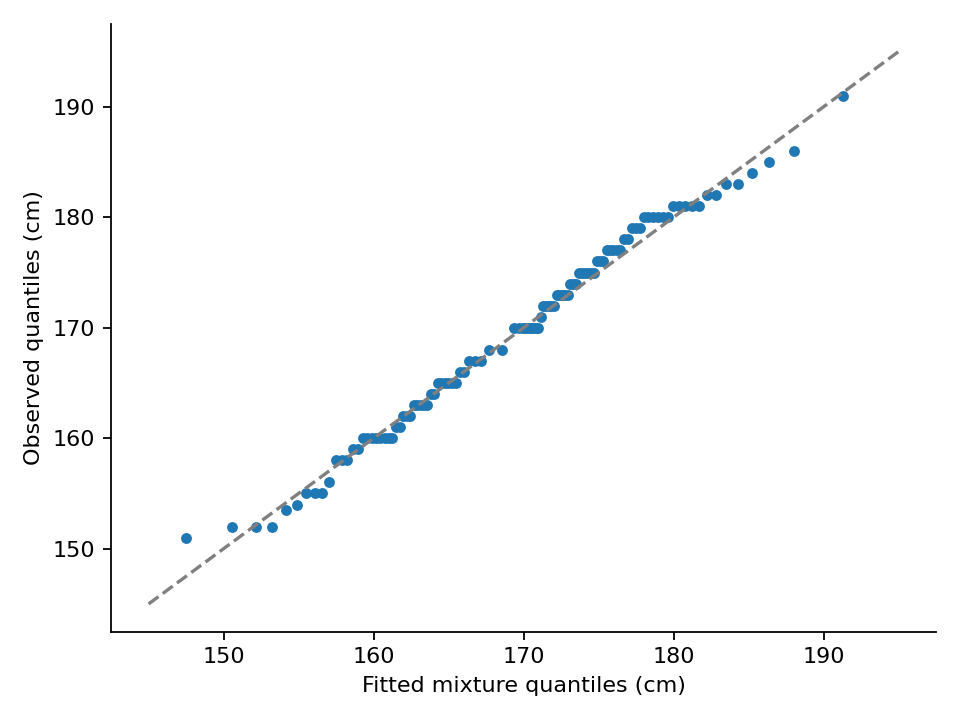
\includegraphics[width=0.72\textwidth,height=0.37\textheight,keepaspectratio]{heights_qq.png}\end{center}

KS statistic $D=0.064523$; Cram\'er--von Mises statistic $W^2=0.070263$. Q--Q plotting positions are $(i-0.5)/n$; mixture quantiles solve $\sum_jw_jF_j(q)=p$ numerically by Brent root finding. Empirical ties remain visible. No goodness-of-fit p-values are reported: fixed-parameter p-values are invalid after fitting to these data. A valid calibration would simulate from the fitted model and refit in each replicate, with rounding modeled if known. Such a parametric goodness-of-fit bootstrap was not executed. The nonparametric bootstrap below assesses uncertainty, not goodness-of-fit p-values.

\clearpage\section*{Bootstrap uncertainty and membership}
An ordinary observation bootstrap resampled 109 rows with replacement, preserving ties and outliers. All seven parameters were refitted jointly, with components relabeled by actual mean. Requested replicates: 200; successful: 200; failed refits: 0. Each replicate used 20 fresh randomized starts plus the primary warm start. There were 0 individual nonconverged starts; a replicate succeeded if at least one start converged. Active constraints occurred in 92.5\% of replicates. The full replicate output includes counts of converged starts and active bounds.

\begin{center}
\small
\begin{tabular}{lr}
\toprule
Number of modes & Bootstrap count\\
\midrule
1 & 9\\
2 & 191\\
\bottomrule
\end{tabular}
\end{center}
Intervals below are the 2.5th and 97.5th percentiles of the successful fits, with their bootstrap median. They describe a constrained, potentially nonregular and weakly identified model, not guaranteed 95\% coverage. The 200 replicates provide a practical uncertainty assessment with appreciable Monte Carlo error; a few modes can change the percentages. Bootstrap refits used fewer starts than the primary fit, so local-optimum error cannot be ruled out.

\begin{center}
\small
\begin{tabular}{lrrr}
\toprule
Quantity & 2.5th percentile & Median & 97.5th percentile\\
\midrule
Mixture mean (cm) & 167.66100 & 169.51564 & 171.11698\\
Mixture SD (cm) & 7.84786 & 9.12214 & 9.96911\\
Lower mode | two modes (cm) & 152.02972 & 162.56417 & 170.02075\\
Upper mode | two modes (cm) & 170.25732 & 176.03247 & 182.12560\\
C1 weight & 0.07850 & 0.44050 & 0.90819\\
C1 location (cm) & 150.85037 & 159.89506 & 174.74534\\
C1 scale (cm) & 1.00000 & 7.72041 & 16.09971\\
C1 alpha & -20.00000 & 1.24040 & 20.00000\\
C1 mean (cm) & 152.68435 & 161.32706 & 169.23782\\
C1 sd (cm) & 0.60413 & 4.90594 & 9.76182\\
C2 weight & 0.09181 & 0.55950 & 0.92150\\
C2 location (cm) & 168.57070 & 179.89258 & 183.69799\\
C2 scale (cm) & 1.00000 & 8.08424 & 15.19268\\
C2 alpha & -20.00000 & -0.20635 & 20.00000\\
C2 mean (cm) & 170.20736 & 175.80156 & 181.10472\\
C2 sd (cm) & 0.60413 & 5.12867 & 9.38796\\
\bottomrule
\end{tabular}
\end{center}
The mode-location rows condition on exactly two modes (191 fits); they exclude unimodal or other fits and must not be read as unconditional mode confidence intervals. The bootstrap bimodal fraction is 0.9550; its simulation standard error is approximately 0.0147.

For each retained observation, the exported posterior membership is
\[
 \tau_{i1}=\frac{wf_1(x_i)}{wf_1(x_i)+(1-w)f_2(x_i)},\qquad
 \tau_{i2}=1-\tau_{i1}.
\]
These are fitted statistical responsibilities, not verified real-world labels
or probabilities of a causal category. The cleaned CSV retains source row
numbers and the exact numerical observations alongside both probabilities.

An independent 32,769-point check of every bootstrap density found 0 discrepancies in mode counts relative to the 4,097-point bootstrap search. Numerical integration verified total mass 1.0000000000, mixture mean and variance, and equality of cleaned observations to the source data.

\clearpage\footnotesize\setlength{\parskip}{4pt}\section*{Quantiles and probability comparisons}
\begin{center}
\small
\begin{tabular}{lr}
\toprule
Mixture quantile & Height (cm)\\
\midrule
q0.10 & 157.64090\\
q0.50 & 170.64597\\
q0.90 & 180.62490\\
\bottomrule
\end{tabular}
\end{center}
Exact computed boundaries, serialized with full precision in JSON, are used consistently for both empirical counts and fitted CDF calculations. The reported rounded table values are for display only. For this continuous model, endpoint point-mass is zero. No contextual threshold $c$ was supplied.

\begin{center}
\small
\begin{tabular}{lrrrrr}
\toprule
Region & Count & Empirical & Fitted & Absolute difference & Relative error (\%)\\
\midrule
Lower tail & 10 & 0.09174 & 0.10000 & 0.00826 & 8.25688\\
Central interval & 86 & 0.78899 & 0.80000 & 0.01101 & 1.37615\\
Upper tail & 13 & 0.11927 & 0.10000 & 0.01927 & 19.26606\\
\bottomrule
\end{tabular}
\end{center}
The intervals use exactly $X<q_{0.10}$,
$q_{0.10}\leq X\leq q_{0.90}$, and $X>q_{0.90}$.
Absolute difference is $|p_{\rm empirical}-p_{\rm model}|$; relative percentage
error is $100|p_{\rm empirical}-p_{\rm model}|/p_{\rm model}$, undefined when
the model probability is zero. These in-sample checks use boundaries estimated
from the same data and are not independent validation.
\section*{Reproducibility and delivered files}
Run from any directory:
\begin{verbatim}
python /path/to/assets/data/fit_heights.py
python /path/to/assets/data/validate_heights.py
python /path/to/assets/data/build_heights_report.py
cd /path/to/assets/data
pdflatex -interaction=nonstopmode -halt-on-error heights.tex
pdflatex -interaction=nonstopmode -halt-on-error heights.tex
\end{verbatim}
Only NumPy, SciPy, pandas and Matplotlib are required for the analysis;
no web connection is needed. The random generator is NumPy default\_rng,
seed 
20261102. All randomized fits and bootstrap resampling consume this generator sequentially, so rerun the whole script to reproduce the sequence. Package versions used:

\begin{center}
\small
\begin{tabular}{lr}
\toprule
Package & Version\\
\midrule
python & 3.11.4\\
numpy & 1.24.3\\
scipy & 1.11.1\\
pandas & 2.0.3\\
matplotlib & 3.7.2\\
\bottomrule
\end{tabular}
\end{center}
The standalone \texttt{heights.tex} uses the four PNG figures in this folder.
Upload the TeX and these PNGs together to Overleaf; it requires no local
absolute paths or external bibliography. Delivered tables: model comparison,
components, probability comparisons, bootstrap replicates and percentile
intervals (CSV). The cleaned data and responsibilities are in
\texttt{heights\_cleaned.csv}. Complete numerical results, bounds diagnostics,
per-start likelihoods, sensitivity fits, versions and input checksum are in
\texttt{heights\_results.json}. The source CSV is unchanged.

Input SHA-256:\par{\scriptsize\texttt{11d5566ab3cff301e6f9ced50c82c3f9\allowbreak b8c9a2b0b978c21fc0b09439cbbd6133}}

\section*{Methods references and unexecuted checks}
The density convention follows the
\href{https://docs.scipy.org/doc/scipy/reference/generated/scipy.stats.skewnorm.html}{SciPy skew-normal documentation}.
The requirement to refit for goodness-of-fit calibration is described in
\href{https://docs.scipy.org/doc/scipy/reference/generated/scipy.stats.goodness_of_fit.html}{SciPy goodness-of-fit documentation}.
No parametric goodness-of-fit bootstrap, dependence-aware bootstrap,
rounded/censored likelihood, external validation or causal grouping analysis
was executed. These require additional computation and/or sampling metadata.
All tables and figures in this report were produced by the executed Python analysis.
\end{document}
